\subsection{Preliminary aging signature: Normalized maximum $NO_x$ reduction}

\begin{figure}[H]
        \begin{minipage}{0.49\textwidth}
                \begin{figure}[H]
                        \centering
                        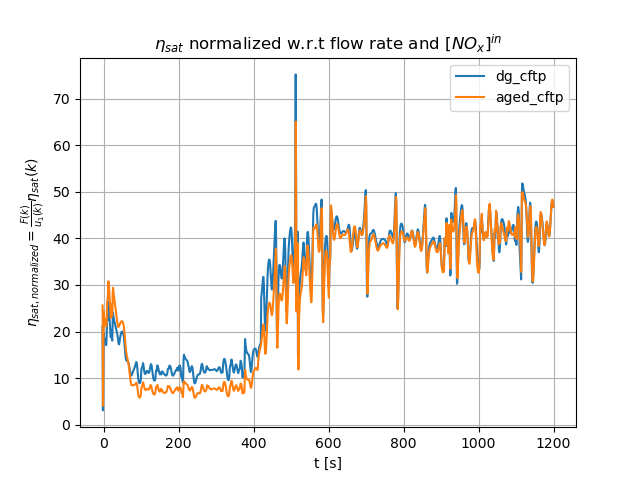
\includegraphics[width=\textwidth]{\froot/figs/14_figs/max_nox/max_nox_aged_cftp.png}
                \end{figure}
        \end{minipage}
        \begin{minipage}{0.49\textwidth}
                \begin{figure}[H]
                        \centering
                        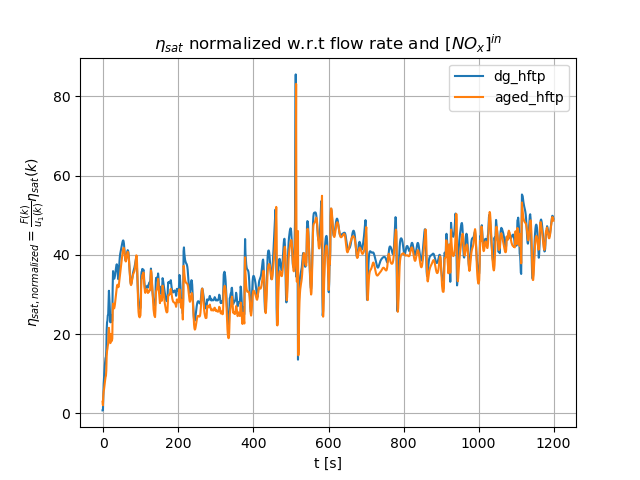
\includegraphics[width=\textwidth]{\froot/figs/14_figs/max_nox/max_nox_aged_hftp.png}
                \end{figure}
        \end{minipage}
        \caption{Maximum $NO_x$ reduction in FTP test data}
\end{figure}

\begin{figure}[H]
        \centering
        \begin{minipage}{0.49\textwidth}
                \begin{figure}[H]
                        \centering
                        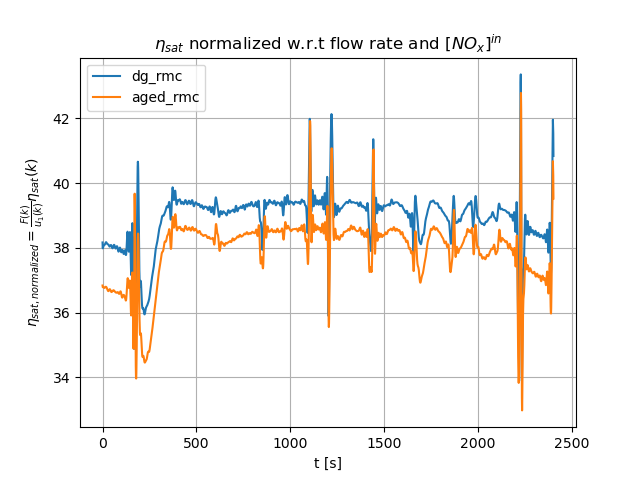
\includegraphics[width=\textwidth]{\froot/figs/14_figs/max_nox/max_nox_aged_rmc.png}
                \end{figure}
        \end{minipage}
        \caption{Maximum $NO_x$ reduction in RMC test data}
\end{figure}

The plots demonstrate clearly the consistent difference between the aged and degreened catalysts. The maximum normalized $NO_x$ reduction is consistently higher for degreened catalyst than that of the aged.
